\documentclass[11pt,oneside,a4paper]{article}
\usepackage{graphicx}
\usepackage{booktabs}
\usepackage{caption}
\usepackage{subcaption}
\usepackage{amsmath}
\usepackage{amsfonts}
\usepackage{amssymb}
\usepackage{lscape}
\usepackage{psfrag}
\usepackage[usenames]{color}
\usepackage{bbm}
\usepackage[update]{epstopdf}
\usepackage[bookmarks,pdfstartview=FitH,a4paper,pdfborder={0 0 0}]{hyperref}
\usepackage{verbatim}
\usepackage{listings}
\usepackage{textcomp}
\usepackage{fancyhdr}
\usepackage{multirow}
\usepackage{tikz}
\usepackage{lipsum}
\usepackage{xcolor}
\usepackage[margin=1in]{geometry}
\newcommand{\hint}[1]{{\color{blue} \em #1}}

\makeatletter
\def\cleardoublepage{\clearpage\if@twoside \ifodd\c@page\else%
\hbox{}%
\thispagestyle{empty}%
\clearpage%
\if@twocolumn\hbox{}\clearpage\fi\fi\fi}
\makeatother

\sloppy
% \widowpenalty=10000
% \clubpenalty=10000

\title{
    \vspace*{0.0mm}
    \LARGE\bf\sf Advanced Topics in \\Communication Networks (Fall 2019)
    \vspace*{10.0mm} \\
    \Large\bf\sf Group Project Report \vspace*{30.0mm}\\
    %
    \Huge\bf\sf Hearding the Elephants: Detecting Network-Wide Heavy Hitters with Limited Resources
    %
    \vspace*{30.0mm} \\
    \normalsize
    %
    \sf Authors:\\[5pt]
    \sf Yannick Merkli\\ [5pt]
    \sf Tim Bohren\\ [5pt]
    \sf Felix Rüssli \vspace*{5mm}\\
    %
    \sf  Advisor: Albert Gran Alcoz \vspace*{5mm}\\
    %
    \sf  Supervisor:  Prof. Dr. Laurent Vanbever \vspace*{20.0mm}\\
    %
    \sf Submitted: Dec 16, 2019\\ [5pt]
    \sf \pageref{lastpage} Pages
}
\date{}

\begin{document}

\begin{figure}
    \includegraphics[width=\textwidth]{figures/eth-nsg-header}
\end{figure}

\maketitle
\thispagestyle{empty}
\raggedbottom
\clearpage

\pagenumbering{roman}

\begin{abstract}
\noindent Detecting heavy hitters (e.g. flows whose packet counts exceed a certain threshold) is an important task for Denial of Service detection, load balancing and traffic routing. Past work has shown how to detect heavy hitters on a single network switch. However, nowadays heavy hitter flows are often \textit{network-wide}, thus detecting them on a single switch is not enough. A flow can enter a network over multiple ingress switches and from each switch's local view, the flow might look normal, whereas from a global view, the flow would be classified as a heavy hitter. Thus, a detection protocol should be distributed to detect flows from a global view \textit{and} detection should still be quick and effective. Further, detecting global heavy-hitter flows inherently poses a trade-off between limitations in network-wide communication and memory resources on the ingress switches and accuracy in detecting heavy hitters.

In this work, we have implemented Herd \cite{anon2019herd}. Herd is a distributed algorithm that identifies network-wide heavy hitters in real time and under constraints on communication and switch memory. The algorithm uses a sample-and-hold technique for flow measurements on ingress switches and probabilistic sampling and reporting of flows. Reporting is done to a central coordinator, which allows for a global view on the network.

\end{abstract}

\clearpage
\setcounter{tocdepth}{2}
\tableofcontents
\clearpage
\pagenumbering{arabic}

\section{Introduction}

Heavy hitters are a minority of flows that are responsible for a majority of packets inside a network. Network operators are interested in spotting them in order to detect and prevent Denial of Service attacks and to maximize the throughput by detecting congestion and failures. Further, heavy hitter detection can also be used for network management such as usage-based pricing or load balancing. To effectively manage and protect networks, heavy hitter detection needs to be quick and efficient. For the following sections, we assume a network to consist of multiple ingress switches through which traffic enters a network. The topology of the inner network is ignored and not important for this work.

Detection of heavy hitters faces several challenges. First of all, heavy hitters don't necessarily enter a network through a single ingress switch and they don't always originate from a single source. As an example, a single host inside a network might be the target of a denial-of-service attack, but traffic targeted towards the host may enter over multiple ingress switches. Local detection on ingress switches will not capture the network-wide view of a flow and will inherently fail at detecting network-wide heavy hitters. Second, network devices are usually limited in their resources, especially when it comes to memory and processing power. This often results in network operators having to choose between high detection accuracy and low processing overhead.

\noindent The problem of a missing network-wide view can be solved by introducing a centralized instance that receives and aggregates partial information from network devices. The burden of heavy hitter detection thus no longer lies on ingress switches but on this centralized instance; usually a general-purpose CPU. The ingress switches only observe and report flows.

\noindent With unlimited memory and processing power on switches and unlimited communication, detecting network-wide heavy hitters would be easy. Each switch could keep track of every single flow, communicate as much as needed with the centralized instance, which can immediately detect based on aggregated information. In reality, switches are highly limited in their memory and processing power. Sending a subset of flow information to a central, general-purpose CPU lifts parts of the limitations on processing power and memory, however new limitations are introduced by the resulting network-wide communication and the fact that a general-purpose CPU is not able to process data at line rate.

%brief description of Herd
Herd \cite{anon2019herd} solves these problems by sampling traffic probabilistically (which saves memory on the switches) and reporting to a central \textit{coordinator} once an observed flow exceeds a certain threshold. This allows for high accuracy in flow detection while operating under the constraints imposed by network devices. The coordinator sees each flow that was reported by an ingress switch and is thus able to combine partial information reported by various ingress switches. This system makes it possible to not only detect local heavy hitters, but also distributed ones, potentially even detecting distributed Denial of Service attacks (DDoS) before they grow to their full potential.


\section{Background and related work}

The basic problem to solve is the following: various flows enter a network and we want to classify them based on a measure that captures each flow's strain on the network (e.g. the packet count). We then want to distinguish \textit{mice flows} (flows without local or global significance) from \textit{elephant flows} (flows with local and global significance).

\noindent There already exist a number of protocols with different approaches to detect elephants. Some existing algorithms, such as NetFlow \cite{claise2004cisco}, sample incoming packets and export them to a central collector. This addresses the constrained switch resources and the flow locality, however these algorithms suffer from temporal 'blind spots' due to low sampling rates and the resulting long delays. Other approaches to heavy hitter detection run streaming algorithms, combined with a compact data structure like a count-min sketch \cite{cormode2005improved} or a bloom filter. These algorithms address the resource constraints of switches, however, they fail to capture network-wide heavy hitters since detection is done on each switch individually.

\begin{figure}
	\centering
	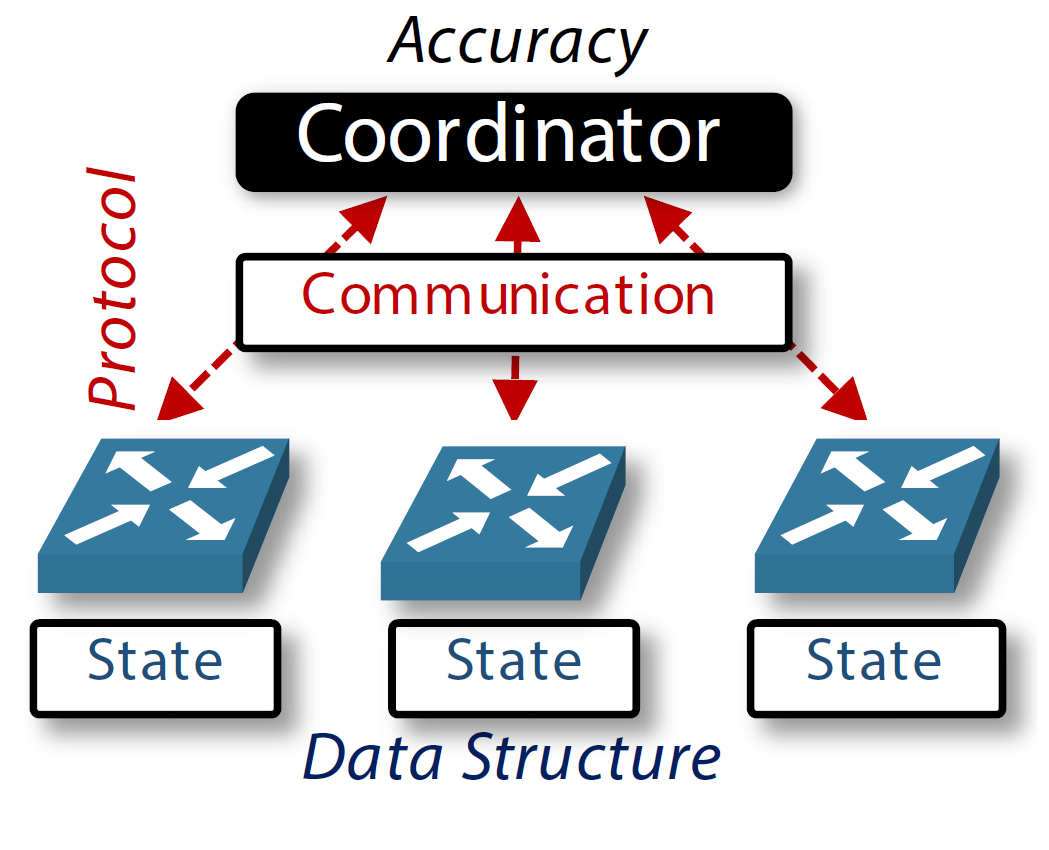
\includegraphics[width=0.5\textwidth,scale=1]{figures/global_local_paper}
	\caption{The Herd switches communicate with the coordinator. \cite{anon2019herd}}
	\label{fig:global_fig}
\end{figure}

\section{Implementation}

We have implemented Herd, as proposed by \cite{anon2019herd}. The Herd architecture consists of local ingress switches and a central coordinator that achieves a global view, as illustrated in figure \ref{fig:global_fig}. Ingress switches probabilistically sample and report incoming flows to the coordinator. For the following sections, we define a flow by the five-tuple $(srcIP, dstIP, srcPort, dstPort, protocol)$. Each flow can be of local and global significance. Additionally to mice and elephant flows, Herd thus introduces two more flow categories to describe all four types of significance: mice, moles, mules and elephants.

\subsection{Herd algorithm} \label{animals}

All flows that enter a network are first classified as mice. Mice are the most common but also the smallest flow type - they don't have local or global significance. When a packet arrives, Herd uses the sample-and-hold algorithm: if the flow to which the packet belongs is already tracked, then its counter is simply increased. Otherwise, we start tracking the flow with sampling probability $s$. With an increasing number of packets belonging to the same flow, the flow's packet count is more likely to be tracked.

\noindent Once a flow is captured by an ingress switch it advances to the next higher tier: the mole. A mole flow is simply a flow whose packet count is tracked by an ingress switch. As such, a mole flow exhibits local significance but no global significance.

\noindent As soon as the packet count of a mole flow on a single ingress switch exceeds the mule threshold $\tau$, the mole flow is reported to the coordinator with report probability $r$. The packet count threshold $\tau$ is introduced for two reasons: First, the coordinator should not waste its memory on every mouse flow that happened to be sampled by the switch. By making sure that each reported flow's packet count exceeds a certain threshold, we ensure to only report globally significant flows that have the potential to  become an elephant, especially when combining reports for the same flow from multiple ingress switches. The other reason is that the network does not have infinite bandwidth, so the switches have to be careful not to congest the network. A flow that has been reported to the coordinator at least once advances from mole flow to mule flow, which means that the flow now has global significance.

\newpage

The coordinator has a global view over all mule flows reported by the ingress switches running Herd, whereas the ingress switches only have a local view since they do not know what other switches observe. Thus the actual classification of elephant flow is solely done by the coordinator. It counts how many reports for a specific flow were received, independently from which switch the report originated from. As soon as the number of reports for a mule flow exceeds the report threshold $R$ the coordinator classifies the flow as an elephant flow, which is synonymous to being a heavy hitter.


\subsection{Locality} \label{locality}
So far it was assumed that all ingress switches have the same probability to observe a flow. However, in real networks flows often exhibit preference for certain ingress switches, meaning certain switches are more likely to observe certain flows. Considering this, we need to increase the mule threshold $\tau$ since every ingress switch observes more packets for fewer flows. A too low mule threshold $\tau$ would result in too many flows being reported to the coordinator, which increases the network-wide communication and increases the number of false positives.

\noindent Herd thus introduces the notion of a \textit{locality parameter} $l_f$, which denotes the number of ingress switches that observe flow $f$. However, tracking the locality on a per-flow level introduces significant overhead. That's why Herd only tracks the locality on a per-group level. A group is defined as

$$g_{src,dst} = \{f | f.srcIP \in src, f.dstIP \in dst\}$$

\noindent where $src$ and $dst$ are /8 IP subnets.

\noindent The new locality parameter $l_g$ now tracks how many ingress switches observe at least one flow $f$ belonging to group $g$. Using the per-group locality parameter $l_g$, the mule threshold $\tau_g$ and the report probability $r_g$ can now be dynamically adapted on a per-group level. Since tracking $l_g$ requires a global view of the network, this is done at the coordinator. For the coordinator to know which ingress switches observe which flows, the ingress switches need to send a message to the coordinator when observing an unexpected (i.e. never before seen) flow. These messages are called \textit{hellos} in Herd.


\subsection{Switch logic} \label{switch}
Herd uses randomness for packet sampling and reporting to the global coordinator. Since P4 doesn't have a random library, we used hashes to 'flip' coins and simulate randomness.
\noindent A  32 bit hash $h$ is calculated from timestamps, the destination IP and the last hash; and if

$$h < int32_{MAX} * probability$$

\noindent the probability is hit. However, the right part of this inequation requires floating point arithmetic, which P4 does not have either. For this reason, the calculation $int32_{MAX} * probability$ is done by the local controller at startup and the resulting \textit{int32} number is then written into a register which can be read by the data plane.

As described in section \ref{locality}, the mule threshold $\tau_g$ and the report probability $r_g$ vary on a per-group level. We thus use a match-action table that maps a group $g_{src,dst}$ to its respective values $\tau_g$ and $r_g$. A second match-action table is used for packet forwarding. We don't care about the internal network structure in this work, so ingress switches simply forward all traffic to an internal aggregator switch, thus this table only has one rule.

The life of a packet when entering an ingress switch looks as follows: the switch first extracts the group $g_{src,dst}$ to which the flow belongs and applies the group values match-action table. In case of a table miss the switch sends a hello message to the local controller, which will then send the hello to the coordinator. The coordinator answers with the locality parameter $l_g$ to the local controller, which will then add a rule to the group values table. For known groups the switch applies the sample-and-hold algorithm. In case the flow is not yet being sampled, we start sampling with sampling probability $s$. If the flow is already being sampled, its counter is increased. In case the counter reaches the group-based mule threshold $\tau_g$, the switch resets the counter and reports the flow with report probability $r_g$. Again, the report will first be sent to the local controller, which will then send it to the coordinator. The communication between data plane and control plane (hellos and reports) is done via copy-to-cpu, where a cloned packet has a CPU header which has six fields: $(srcIP, dstIP, srcPort, dstPort, protocol, flow\_count)$.

The counters counting the number of seen packets per flow are stored in a multi-stage hash table with three stages that decrease in size. The index of the flow counter in the hash table is determined by hashing the flow five-tuple $(srcIP, dstIP, srcPort, dstPort, protocol)$. Register entries are 64 bit wide. The lower 32 bit store the flow count. The upper 32 bit store a hash (with a different hash function) of the flow five-tuple (flow key) which is used to detect hash collision. In case of a hash collision, the next hash table is considered. Note that the width of the registers can be chosen smaller than 64 bit. In case of few flows, hash collision become less likely and a smaller hash space for the flow key is acceptable. Further, the flow counter will never become much larger than $\tau_g$ since the counter is reset to zero when a report is sent. We decided to use 64 bit wide registers to make sure that hash collisions are unlikely, even for large numbers of flows.

\subsection{Herd Controller} \label{controller}

A Herd controller is running on each ingress switch. The controller's main task is to communicate with the coordinator and write rules into the group values match-action table.

\noindent During the startup phase, the controller cleans all hash tables, writes the sampling probability to the data plane, fills the forwarding table and connects to the coordinator RPC server. To handle communication between data plane and control plane, the controller sniffs on the copy-to-cpu interface and unpacks each received cloned placket. Each clone packet includes a CPU header, stating the flow five-tuple and the packet count for the flow (flow count). The controller determines, based on the flow count, whether the received message is a hello or report: hellos have a flow count of zero whereas reports have a flow count larger than zero. The controller then sends the hello or report to the coordinator by initiating a remote procedure call, including the flow and the switch name as arguments.

\noindent When multiple packets of a flow belonging to a never before seen group $g$ arrive at an ingress switch, it is possible that the data plane sends multiple hellos due to delayed writes into the group values table. The original Herd paper \cite{anon2019herd} would just send all hellos to the coordinator. We decided, in order to avoid overloading the network with hellos, to adapt the Herd controllers to keep track of the flows for which a hello was already sent. This way, each controller only sends one hello per flow to the coordinator and we don't overload the network or the coordinator with unnecessary hello messages.

\noindent Additionally to a sending, the Herd Controller also needs to receive messages from the coordinator. Upon receival of $l_g$, the controller calculates the mule threshold as $\tau_g = \frac{\epsilon \cdot T}{l_g}$ ($\epsilon$ is an approximation factor on the communication) and the reporting probability as $r_g = \frac{1}{l_g}$, where $r_g$ is then transformed into an \textit{'int32-probability'} (see section \ref{switch}). The controller then writes $\tau_g$ and $r_g$ into the group values table with the group $g$ $(for \; f \in g)$ as match key and $\tau_g, r_g$ as action parameters.


\subsection{Herd controller - coordinator communication} \label{communication}

The communication model specified by Herd has the following three important characteristics: First, the coordinator needs to provide a service to one or many Herd controllers, which request the service. Second, communication should be asynchronous since hellos and reports can be generated anytime. Waiting for synchronous communication rounds would introduce additional delay, which would worsen detection accurcay. Last but not least, the communication needs to be two-way, since the coordinator needs to respond to hellos.

We decided to use a remote procedure call (RPC) protocol, since it fulfills all three mentioned characteristics. The coordinator server runs an RPC service that implements two exposed methods, $send\_hello$ and $send\_report$, which can be invoked by Herd controllers. The communication from coordinator to Herd controller is implemented through a callback. When invoking $send\_hello$, a Herd controller passes the name of the switch and a callback function, which will be registered at the coordinator and called once the locality parameter $l_g$ is sent back.


\subsection{Coordinator} \label{coordinator}
The central coordinator receives and handles hellos and reports sent by Herd controllers and sends back the locality parameter $l_g$. The coordinator further keeps track of the number of sent reports and classifies flows as heavy hitters.

\noindent When a hello arrives, the coordinator first registers the callback for the sending switch. It then extracts the group $g$ from the flow five-tuple and looks up the locality parameter $l_g$. The coordinator further keeps track of which switches observe at least one flow belonging to group $g$. In case the number of switches that see a group doubled, $l_g$ is updated and sent to each switch that observes $g$. Otherwise, $l_g$ is only sent to the switch sending the hello.

Handling reports is rather simple. The coordinator simply counts the number of received reports for each flow. As soon as the number of reports reaches the reporting threshold $R$, the flow is put into a heavy hitter set and thus promoted to an elephant flow.

\subsection{Tuning the parameters} \label{tuningparameters}


Up until now it was assumed that the approximation parameter $\epsilon$, the sampling probability $s$ and the report threshold $R$ were given, however, they need to be selected carefully, since a poor choice of parameters may lead to a decrease in Herd performance. Parameter selection needs to consider the constraints on switch memory $S$ and communication budget $C$ and should not be done in isolation - optimizing for one single parameter while ignoring the rest could decrease detection accuracy. We have implemented an algorithm, proposed by the Herd paper \cite{anon2019herd}, that jointly optimizes for the three aforementioned parameters, given a packet trace $D$ as training data.

The basic idea behind the tuning algorithm is simulating the Herd protocol. One starts with specifying the memory budget $S$ per switch, the communication budget $C$ per switch and the global threshold $T$, i.e. the number of packets of a flow for which a flow is labeled a heavy hitter. The algorithm first empirically determines the highest possible sampling probability $s$ of the sample-and-hold algorithm, given the memory constraint $M$. It then iterates through possible approximation factors $\epsilon$ and returns the parameters which maximize the accuracy. For each iteration, the algorithm first configures the mule threshold $\tau$, the report probability $r$ and the report threshold $R$, given the found sampling probability $s$, the communication constraint $C$ and the $\epsilon$ for the current iteration. Based on the mule threshold, it then finds all mule flows in $D$. Finally, based on the set of mule flows $U$, the report probability $r$ and the report threshold $R$, the algorithm calculates how many reports each flow would have generated in expectation and labels it as a heavy hitter if the estimated report count exceeds $R$. Finally, the set of detected heavy hitters is compared with a precomputed real heavy hitter set and the F1 score is calculated. In the end, the parameter set with the highest F1 score is returned.

We tried to implement the tuning algorithm as specified by the Herd paper, however the authors omitted many crucial details, such as how and based on which measure the accuracy is determined. Further, they do not explain how they simulate the labeling of mole and mule flows. We thus had to make several assumptions during the implementation of the tuning algorithm. In the end, we were not able to reproduce the results that the paper was able to achieve with the tuning parameters algorithm. We were able to simulate the Herd algorithm, however we got F1 scores in the range of $10\% - 50\%$, which is clearly not optimal.


\subsection{Full hash tables} \label{special}

Flow counters are stored on each ingress switch in a multi-stage hash table. In case of full hash tables, Herd proposes to just send all packets of the flow to the coordinator which introduces significant delay and communication cost. Further, the Herd paper does not specify what the coordinator should do with the packets.

In our implementation, we handle full hash tables differently. Instead of sending all packets to the coordinator, the data plane sends an error message to the controller, indicating full hash tables. The controller will subsequently reset the hash tables. We argue that due to the fact that counters of large flows are reset back to zero anyways in case of a report, this leads to a minor decrease in accuracy. In the worst case, we reset the hash table when the packet count of flow $f \in g$ is $n_f \approx \tau_g$. The flow needs to be resampled in order for it to be counted again. Thus, in expectation, the number of missed packet counts is roughly $\tau_g+\frac{1}{s}$, which can be compared to losing one report. For overall detection, this is reasonable, especially since usually the report threshold is $R > 10$.

\subsection{Challenges} \label{challenges}

We faced several challenges during the implementation and evaluation of Herd. The main challenge was limitations imposed by running Herd in a simulated environment and not in hardware. An important part of classification accuracy is how fast we can write or update an entry in the group values table. Whenever an incoming packet on the switch creates a table miss in the group values table, the switch will send a hello in order to fill the table. The total delay between the switch sending a hello and the controller writing the table rule is

$$\Delta t_{hello_f} = t_{DC} + 2*t_{CC} + t_{table\_write} + \epsilon$$

\noindent where $t_{DC}$ is the delay introduced by the data plane to control plane communication (digests or copy-to-cpu), $t_{CC}$ is the delay introduced by the controller-coordinator communication, $t_{table\_write}$ is the time it takes to write into a match-action table and $\epsilon$ are negligible processing delays. Every packet belonging to flow $f \in g$ that arrives during $\Delta t_{hello_f}$ will not be sampled and the higher the sending speed, the more packets belonging to $f$ will arrive during $\Delta t_{hello_f}$. 

Further, we observed that the mininet starts dropping digest/copy-to-cpu messages at packet sending rates exceeding 350 packets per second (pps) and the load balancer started dropping packets at sending rates exceeding 8000 pps. We were thus limited to sending rates of 300 pps, which made evaluations over large pcap files take a long time. For a sending rate of 300 pps, a packet trace consisting of five million packets would take 4.6 hours. When running multiple evaluation runs, the total evaluation would easily take days. We thus limited our evaluation to packet trace with 100'000 and 400'000 packets. Note that these limitations only apply to simulations; in real hardware, the data plane to control plane communication would work over a direct link, which would remove the bottleneck. In that case, the main delay would then come from the controller to coordinator communication. \newline 

\noindent Another challenge we faced was that the Herd paper \cite{anon2019herd} was often times very unspecific and omitted crucial details (see section \ref{original_paper}).


\subsection{Assessment of the original paper} \label{original_paper}

Unfortunately, the Herd paper \cite{anon2019herd} has several weaknesses which made implementing it rather challenging. The paper is often extremely vague and omits crucial details. The authors stress the importance of tuning parameters such as the sampling probability $s$, the report threshold $R$ or the approximation factor $\epsilon$, to that end they propose a tuning parameters algorithm which intends to simulate Herd and find an ideal parameter set, given a packet trace as training data. Although providing part of the algorithm in pseudo code, many details are neglected, which required assumptions from our side. In the end, we were not able to reproduce a meaningful set of parameters using their tuning algorithm.

Considering the importance the paper puts on finding the right parameters, the authors blatantly omit mentioning which parameters were used for their evaluation. Since we were not able to reproduce the paper's tuning parameter algorithm, we thus had to find an optimal set of parameters by evaluating Herd in a mininet over multiple parameters, which eventually allowed us to at least find a locally optimal parameter set.

A further critique from our side is the dependence on training data of the tuning parameters algorithm. When using a certain packet trace as training data, inherent assumptions about the target traffic are made, thus introducing the need for representative packet traces. This is generally difficult, since internet traffic varies widely.

\section{Evaluation}

\subsection{Topology} \label{topology}

For the evaluation, we used the topology displayed in figure \ref{fig:topology_fig}, as proposed by the Herd paper \cite{anon2019herd}. The topology is composed of $k=10$ edge (ingress) switches $s_1 - s_{10}$, representative of a wide-area network. Each ingress switch is running Herd with its Herd controller communicating with the coordinator. The host $h_1$ represents an external host which sends traffic towards an internal host $h_2$, crossing the ingress switches $s_1 - s_{10}$. As outlined in section \ref{locality}, flows usually show affinity for a limited number of ingress switches. As proposed by the paper, each flow will enter the network over $l = 2$ ingress switches $s_{primary}$, $s_{secondary}$, where $P[s_{primary}] = p = 0.95$ and $P[s_{secondary}] = 1-p = 0.05$. The two ingress switches are selected based on the hash of the source IP address. In order to distribute flows over ingress switches, we added a load balancer switch that extracts the source IP of each packet, calculates a hash and sends the packet to $s_{primary}$ with $0.95$ probability and to $s_{secondary}$ with $0.05$ probability. Probabilistic coin flips are again implemented as explained in section \ref{switch}. Additionally, we added an aggregating switch to the topology, which basically collects all traffic that the ingress switches forward and then sends it to the internal host $h_2$. Both, the load balancing switch and the aggregating switch have their own controllers that run at initialization time and write forwarding rules into match-action tables.


\noindent To generate a sizable amount of traffic on the sending host $h_1$ we use CAIDA's anonymized internet packet traces from 2016, the same packet traces the Herd paper used. Due to the problems specified in \ref{challenges}, we sized down the packet traces to pcap files with 100'000 or 400'000 packets. Instead of Python's scapy library, which only achieves very low sending rates, we used \textit{tcpreplay} to send packets on host $h_1$. \textit{tcprewrite} was used in order to add the correct source and destination MAC addresses (i.e. the MAC address of the sending interface on $h_1$ and the MAC address of the receiving interface on the load balancer $lb$) to the packets in the pcap file.


\begin{figure}
	\centering
	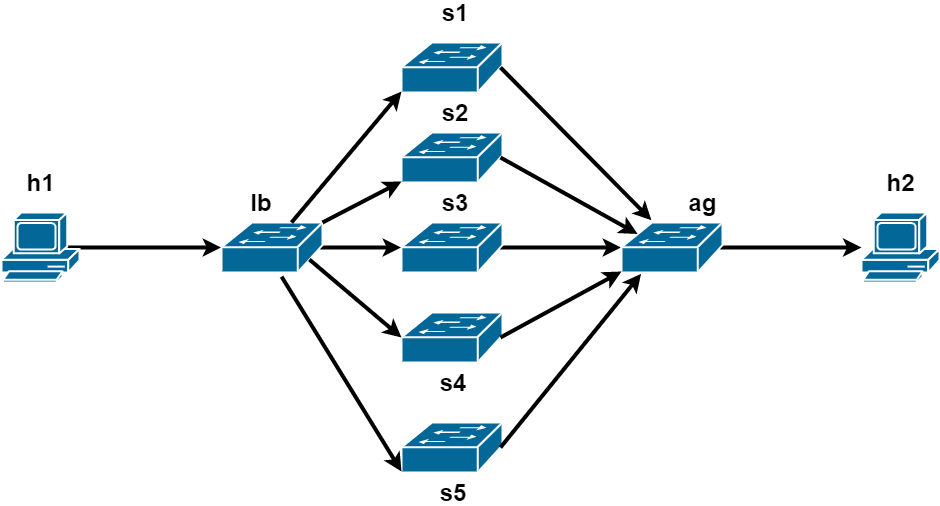
\includegraphics[width=0.7\textwidth]{figures/Herd_topology}
	\caption{Evaluation topology: $h_1$ sends traffic towards $h_2$, crossing the ingress switches $s_1 - s_{10}$, which all run Herd}
	\label{fig:topology_fig}
\end{figure}

\subsection{Detection accuracy} \label{accuracy}

In the following evaluations, we look at detection accuracy, meaning out of all flows that Herd labeled as heavy hitters, how many do we classify correctly (true positive), how many do we mistakenly classify as heavy hitters (false positive) and how many actual heavy hitters don't we classify as such (false negative). Note that by \textit{positive} we always mean \textit{heavy hitter}. We look at the accuracy measures F1 score, precision and recall.

In order to calculate these accuracy measures, we need to know the actual heavy hitters of a packet trace. This is done by parsing all packets of a pcap file and calculating the flow count for each flow. The heavy hitter set is the set of flows whose flow counts exceed a global threshold $T$. Setting $T$ is a design choice that depends on the network and traffic specifics. The Herd paper used the $99.99^{th}$ percentile flow count in the packet trace. We decide to use the $99^{th}$ percentile since we use smaller packet traces and a smaller global threshold will result in more heavy hitter flows. Accuracy is then simply calculated by comparing the 'real' heavy hitter flows with the 'found' heavy hitter flows (which are returned by the coordinator).


\subsection{Herd performance over different sampling probabilities} \label{sampling_probability_evaluation}

One of the main ideas behind Herd is to probabilistically sample flows such that network devices don't need to keep track of every flow they observe, which would be infeasible for large number of flows due to the limited memory on network devices. The sampling probability $s$ dictates how many states a switch will eventually have to track, i.e. the lower the sampling probability, the lower the number of required states. We thus evaluated Herd for different sampling probabilities, using an approximation factor of $\epsilon = 0.1$, which proved to be optimal (see section \ref{epsilon_evaluation}). As seen in figure \ref{fig:sampling_prob_graph}, for sampling probabilities $s > 0.1$, the F1 score stays in the range $[85\%, 90\%]$. Herd with $s = 0.1$ is thus able to achieve the same detection accuracy as an algorithm that samples every single flow ($s = 1$), which needs \textit{ten times} as much memory per switch. The claim of the paper that Herd is able to achieve high accuracy under memory constraints was thus reproduced by us. Our achieved F1 score is $5\% - 10\%$ lower than found by the Herd paper. We argue that the slightly lower detection accuracy (F1 score) is caused by delays introduced by running evaluations in a simulated environment.

One thing worth discussing is the decrease in precision for larger sampling probabilities. We reason that for larger sampling probabilities, more flows are being sampled while the report threshold $R = \frac{1}{\epsilon}$ stays constant, thus more flows will be wrongly classified as heavy hitters, resulting in more false positives, which decreases precision. A possible adaption to Herd would be to adjust the report threshold $R$ with the sampling probability.


\subsection{Herd performance over different approximation factors} \label{epsilon_evaluation}

The approximation factor $\epsilon$ influences the local mule threshold $\tau_g = \frac{\epsilon \cdot T}{l_g}$ and the report threshold $R = \frac{1}{\epsilon}$, which both directly influence heavy hitter detection, thus $\epsilon$ should be selected carefully. Ideally, one would jointly search for an ideal parameter set using the tuning parameters algorithm, which the Herd paper did. However, as mentioned in section \ref{tuningparameters}, we were not able to reproduce their results. We thus used the results from \ref{sampling_probability_evaluation}, chose a sampling probability of $s = 0.2$ and then evaluated over a range of $\epsilon \in [0.001, 1.0]$. As seen in \ref{fig:epsilon_graph}, the optimal $\epsilon$ is at $\epsilon = 0.09$ with an F1 score of $89\%$. The results generally align with the the Herd paper, however we found a much smaller band of ideal $\epsilon$.

\begin{figure}
	\centering
	\begin{subfigure}{.5\textwidth}
		\centering
		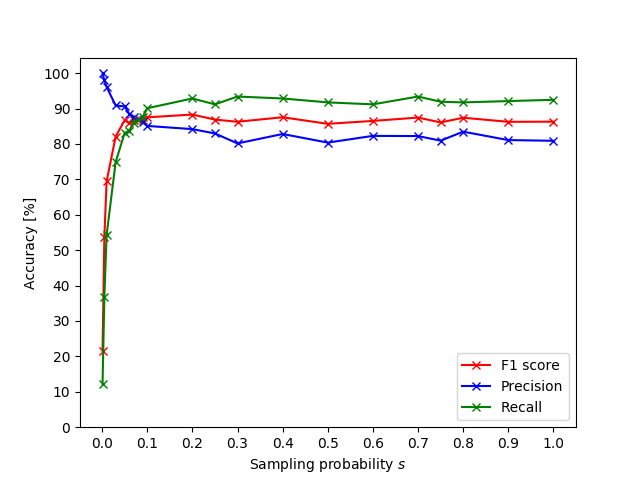
\includegraphics[width=\linewidth]{figures/sampl_prob_400k_e0_1_re}
		\caption{Evaluation over sampling probabilities. \newline
			approximation factor $\epsilon = 0.1$, 400'000 packets, \newline
			 $T = 91$, report threshold $R = \frac{1}{\epsilon} = 10$}
		\label{fig:sampling_prob_graph}
	\end{subfigure}%
	\begin{subfigure}{.5\textwidth}
		\centering
		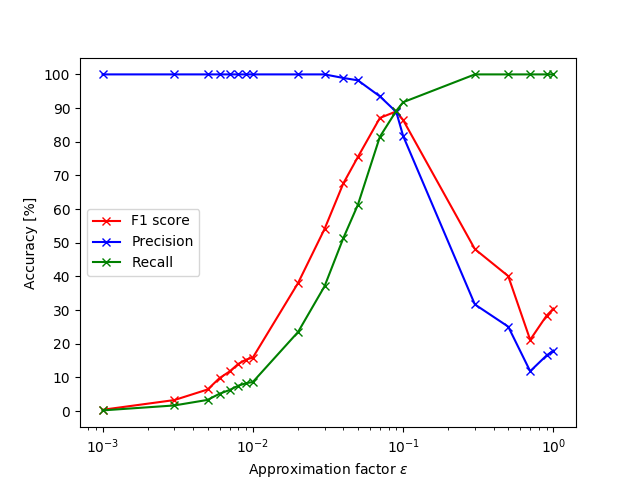
\includegraphics[width=\linewidth]{figures/epsilon_400k_s0_2_re}
		\caption{Evaluation over approximation factors $\epsilon$. \newline
			sampling probability $s = 0.2$, 400'000 packets, \newline
			$T = 91$, report threshold $R = \frac{1}{\epsilon}$}
		\label{fig:epsilon_graph}
	\end{subfigure}
	\caption{Herd performance with varying parameters $s$ and $\epsilon$}
\end{figure}


\subsection{Herd performance against other approaches} \label{other_approaches_evaluation}

To finish our evaluation we compared our Herd performance against the alternative solutions mentioned in \cite{anon2019herd}, namely a probabilistic reporting (PR), a probabilistic sampling (PS) and a strawman solution. The strawman counts every flow and reports all counters at the end of a window. The PS technique does sample a packet with a given sampling probability and reports all samples. The PR technique counts every flow and reports all flows that reach a given threshold with report probability $r = \frac{1}{k}$ (where $k$ is again the number of ingress switches).
\newline We compared the memory usage and the communication needed by the four solutions for the 100'000 packets dataset, which contains 23100 unique flows. As Figure \ref{fig:states_required} shows the memory needed by each technique for different sampling probability values in a range where all techniques get similar F1 scores. As one can see, Herd requires drastically less memory than the other approaches apart from PS, which is stateless. Herd beats the other approaches, even tho we only used the lower bound of $memory\_required \geq \#flows$. The states required by Herd are also highly dependant on the sampling probability and we can approximate them as: $memory\_required = \#flows * sampling\_probability * L$, where $L$ is the number of ingress switches that see the same flow ($L = 2$ in our test setup). Depending on $s$ we have a memory usage reduction of 50\% to 80\%, which is even more than the original paper proposed. \newline

\begin{figure}%[hb]
	\centering
	\begin{subfigure}[t]{.53\textwidth}
		\centering
		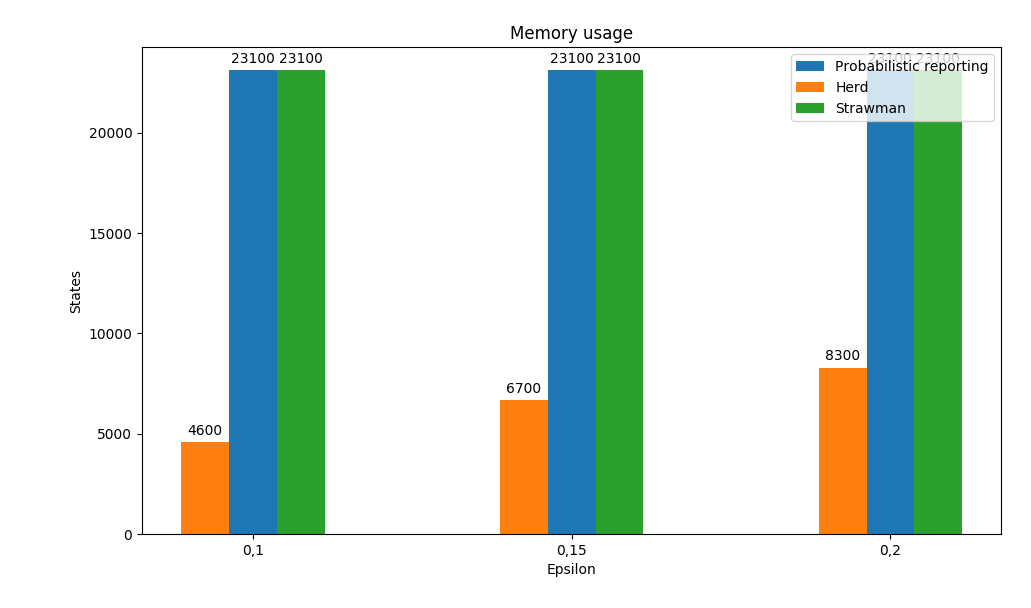
\includegraphics[width=\linewidth]{figures/required_states}
		\caption{Evaluation of the states required for \newline
			different sampling probabilities $s$, 100'000 packets}
		\label{fig:states_required}
	\end{subfigure}%
	\begin{subfigure}[t]{.5\textwidth}
		\centering
		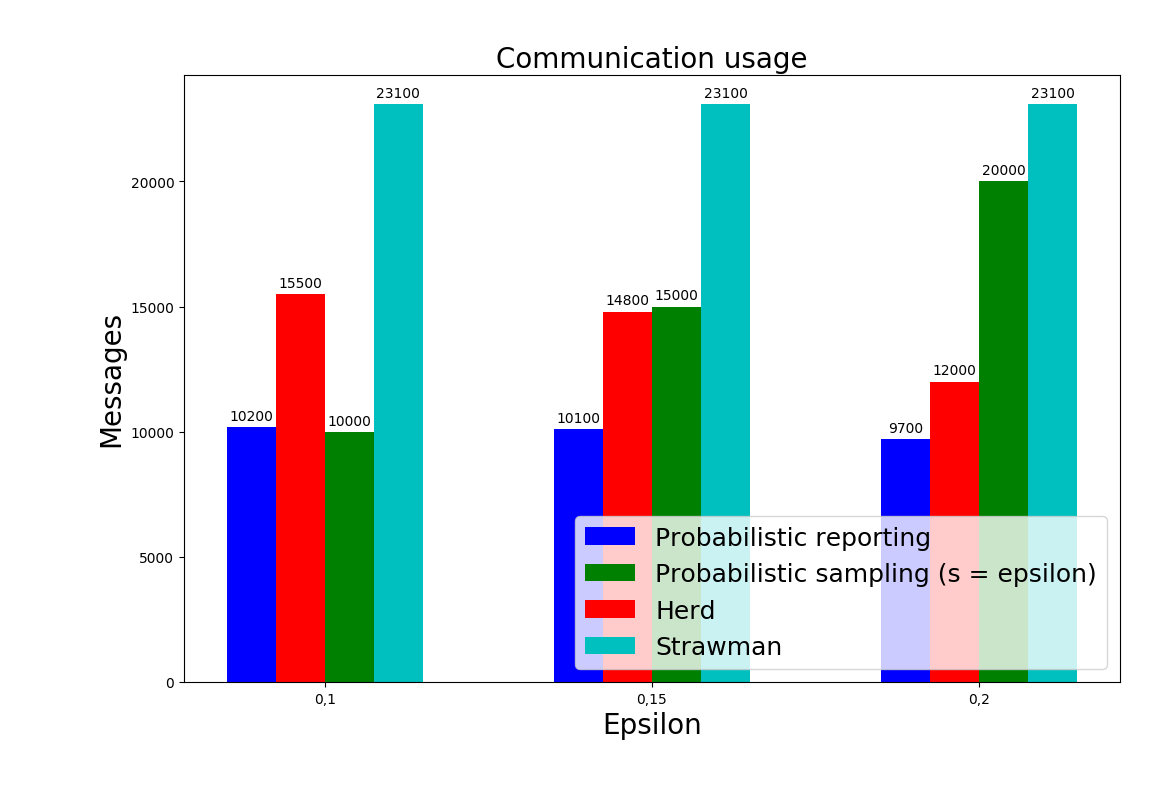
\includegraphics[width=\linewidth]{figures/generated_messages}
		\caption{Evaluation of the generated messages for \newline 
			different approximation factors $\epsilon$, 100'000 packets}
		\label{fig:messages_generated}
	\end{subfigure}
\caption{Herd performance against other approaches}
\end{figure}

\newpage

\noindent The comparison between the bandwidth usage of the different approaches is done by comparing how many messages each approach generates. From figure \ref{fig:messages_generated}, which shows the generated messages for different $\epsilon$ values that lead to similar F1 scores (for probabilistic sampling we set the sampling probability equal to $\epsilon$), we can make several observations:

\begin{enumerate}
	\setlength{\itemsep}{0pt}
	\setlength{\parskip}{0pt}
	\item Herd is substantially better than the strawman approach, which is approximated by it's lower bound $messages\_generated \geq \#flows$.
	
	\item Herd scales better than PS, as we can reduce the needed communication via the approximation factor $\epsilon$ and the report probability $r$. PS can only reduce the sampling probability to generate fewer messages which quickly leads to deteriorating F1 scores.
	
	\item  The difference between Herd and probabilistic reporting mainly stems from the hello messages overhead, which was around 7000 for our setup. Since we can upper bound the generated messages by $hellos\_generated < \#groups * k$, and the number of groups grows much slower than the number of flows, this overhead should become less significant with bigger datasets or larger time windows. Therefore we can conclude that Herd and probabilistic reporting will stay competitive in regard to communication, while Herd has a clear advantage since it requires less memory.
\end{enumerate}

\section{Conclusion}

We successfully reimplemented Herd, a distributed heavy hitter protocol as proposed by \cite{anon2019herd}. We further implemented an evaluation topology, including a load balancer and aggregating switch, and an automated evaluation procedure which automatically initializes a mininet, sends traffic from a host and evaluates heavy hitter detection performance.

\noindent Our main findings generally align with those of the Herd paper. Herd is able to detect heavy hitters with high accuracy while under memory and communication constraints. Due to the constraints imposed by running the evaluation in a simulated environment, our detection accuracy was generally lower than the one in the Herd paper and we were only able to evaluate at low sending rates and thus with small packet traces, which limits  real-world significance.

Future research could go towards improving the parameter tuning. The current implementation, as proposed by \cite{anon2019herd}, depends on training data. Finding representative packet traces is rather difficult since internet traffic can vary widely. An improved protocol could dynamically adjust parameters such as the report treshold and the approximation factor.


\label{lastpage} % this must stay here
\clearpage
\addcontentsline{toc}{section}{References}
\bibliographystyle{acm}
\bibliography{refs}

\clearpage
\appendix
\pagenumbering{Roman}

\section{Group organization}

\paragraph{Yannick Merkli}
\begin{itemize}
	\item Implemented the coordinator and the RPC communication
	\item Wrote the Herd controller algorithm
	\item Implemented the load balancer switch and the aggregator switch in P4
	\item Evaluated Herd and wrote report for \ref{sampling_probability_evaluation}, \ref{epsilon_evaluation}
\end{itemize}


\paragraph{Tim Bohren}
\begin{itemize}
	\item Implemented the Herd switch in P4
	\item Wrote the data plane - control plane communication (copy-to-cpu)
	\item Implemented the automatic evaluation script
	\item Evaluated Herd and wrote report for \ref{other_approaches_evaluation}
\end{itemize}

\paragraph{Felix Ruessli}
\begin{itemize}
	\item Wrote the tuning parameter algorithm
	\item Wrote the report
	\item Created the presentation
\end{itemize}

\end{document}
